\chapter{Introduction}
\label{chap:context}
In this dissertation I present SFL-explorer: a tool to demonstrate how functional programming languages are evaluated, allowing users to gain a valuable intuition of these languages. It is an open source web based tool, available for download and offline use as a PWA (Progressive Web App, see \ref{bg:pwa}). 

SFL-explorer takes the form of a functional language (\ac{SFL}), packaged with two interfaces that allows users to observe the process of evaluation of a term as a series of step by step or multi-step reductions, and control the order that sub-terms are evaluated. These interfaces are a \ac{CLI} and a web application. The ultimate goal of this project was to make a tool that makes learning and teaching the basics of functional programming easier. There are two groups of people the project is designed to be of interest to:
\begin{itemize}
    \item Those involved in learning functional languages. These could be students of a university course, or anyone interested in the topic. 
    \item Those involved in teaching functional languages, as part of a university course or otherwise.
\end{itemize}

\section{The Language}
The language itself is not meant to be the main interest for the users of this system. It is designed to be fairly generic, with syntax and semantics similar to popular functional languages, so that users can take their understanding from using SFL-explorer and apply it to these languages. \ref{tab:fac_2_table_input} is an example program in the language, to find the factorial of 2. The relevant prelude functions are included for clarity.

\begin{figure}[h]
\begin{lstlisting}[language=SFL]
if :: Bool -> a -> a -> a
if cond then_branch else_branch = match cond {
  | true -> then_branch
  | false -> else_branch
}

fac :: Int -> Int
fac n = if (n <= 1) (1) (n * (fac (n - 1)))

main :: Int
main = fac 2
\end{lstlisting}
\caption{An example SFL program. Evaluation is shown \ref{tab:fac_2_table}}
\label{tab:fac_2_table_input}
\end{figure}

\ref{tab:fac_2_table} is a table showing the evaluation of this function in lazy mode by the system. The `Prompt` column shows what the user is presented with as a button to make progress. The first prompt entry at row $0$ is empty, as it represents the starting program state. This table is generated dynamically as the user progresses through the given program.  


\begin{figure}[t]
    \centering
    \begin{tabular}{|l|p{5cm}|l|}
\hline
    Step & \textbf{Prompt} & \textbf{Main Expression Afterwards} \\ \hline
    0 &     \  & \begin{lstlisting}[language=SFL_unboxed]
fac 2
\end{lstlisting}\rule[-2ex]{0pt}{0pt} \\ \hline
     1 & Apply function `fac' to 2 & \begin{lstlisting}[language=SFL_unboxed]
if (2 <= 1) 1 (2 * (fac (2 - 1)))
\end{lstlisting}\rule[-2ex]{0pt}{0pt} \\ \hline
    2 &\makecell[l]{Apply function if to (2 <= 1), 1 \\\ \ and (2 * (fac (2 - 1)))}
    & \begin{lstlisting}[language=SFL_unboxed]
match (2 <= 1) {
  | true -> 1
  | false -> 2 * (fac (2 - 1))
}
\end{lstlisting} \\\hline
    3 & Apply inbuilt <= to `2' and `1'  & \begin{lstlisting}[language=SFL_unboxed]
match (false) {
  | true -> 1
  | false -> 2 * (fac (2 - 1))
}
\end{lstlisting} \\\hline
     4 & Match to pattern `false' & \begin{lstlisting}[language=SFL_unboxed]
2 * (fac (2 - 1))
\end{lstlisting}\rule[-2ex]{0pt}{0pt} \\\hline
    5  & \makecell[l]{Apply function fac to (2 - 1)}
    & \begin{lstlisting}[language=SFL_unboxed]
2 * (if ((2 - 1) <= 1) 1 ((2 - 1) 
    * (fac ((2 - 1) - 1))))
\end{lstlisting} \\\hline
     
    6 & \makecell[l]{Apply function if to \\\ \ ((2 - 1) <= 1), 1 and \\\ \ ((2 - 1) * (fac ((2 - 1) - 1)))}
    & \begin{lstlisting}[language=SFL_unboxed]
2 * match ((2 - 1) <= 1) {
  | true -> 1
  | false -> (2 - 1) * (fac ((2 - 1) - 1))
}
\end{lstlisting} \\\hline
     
     7  & \makecell[l]{Apply inbuilt - to 2 and 1}
    & \begin{lstlisting}[language=SFL_unboxed]
2 * match (1 <= 1) {
  | true -> 1
  | false -> 1 * (fac (1 - 1))
}
\end{lstlisting} \\\hline

  8  & \makecell[l]{Apply inbuilt <= to 1 and 1}
    & \begin{lstlisting}[language=SFL_unboxed]
2 * match (true) {
  | true -> 1
  | false -> 1 * (fac (1 - 1))
}
\end{lstlisting} \\\hline
     
     9 & \makecell[l]{Match to pattern true}
    & \begin{lstlisting}[language=SFL_unboxed,aboveskip=0pt,belowskip=0pt]
2 * 1
\end{lstlisting}\rule[-2ex]{0pt}{0pt} \\\hline

   10 & \makecell[l]{Apply inbuilt $*$ to 2 and 1}
    & \begin{lstlisting}[language=SFL_unboxed,aboveskip=0pt,belowskip=10pt]
2
\end{lstlisting}\rule[-2ex]{0pt}{0pt}\\\hline
\end{tabular}
    \caption{A table showing how the system leads a user through the step by step evaluation of the program shown in Figure \ref{tab:fac_2_table_input}}
    \label{tab:fac_2_table}
\end{figure}

The user is provided with messages telling them what the next step that they can make is. Additionally, there is a `free choice' mode where users are presented with the options for progress, and they can choose which one is taken.

\section{COMS10016: Imperative and Functional Programming at the University of Bristol}
\label{COMS10016}
In the first year of most computer science programs at the University of Bristol, students take the module \href{https://www.bristol.ac.uk/unit-programme-catalogue/UnitDetails.jsa?unitCode=COMS10016}{COMS10016}, a combined imperative and functional programming module. This is many students first encounter with both of these types of programming. In the functional part of this unit, students are taught Haskell. The unit material is presented to students through a very effective lecture series, supplemented by weekly worksheets that students have the opportunity to work through in labs attended by the lecturers, as well as some teaching assistants. Two of the lecturers in this unit are Jess Foster and Samantha Frohlich. 

\begin{quote}
`The aim [of the functional portion of the unit] is to introduce types and functions. Important principles include datatypes, evaluation order, higher-order functions, and purity' \cite{COMS10016}
\end{quote}

\noindent I acted as a teaching assistant in the labs for two academic years. My role was to answer students questions about functional languages or the worksheets they were given. The inspiration for this project came from my experience struggling to explain key functional programming concepts. 

\section{Agile Development Lifecycle}
The project followed a development lifecycle inspired by Agile principles\cite{agilemanifesto2001}, structured into four iterative phases. Each phase built upon the last, integrating evaluation and feedback to continuously and rapidly refine the features and the UI/UX of the system. 

Each phase was further subdivided into four phases:

\begin{itemize}
    \item \textbf{Requirements Gathering}
    \item \textbf{Design and Research}
    \item \textbf{Implementation}
    \item \textbf{Evaluation}
\end{itemize}

\begin{figure}[t]
    \centering
    \fbox{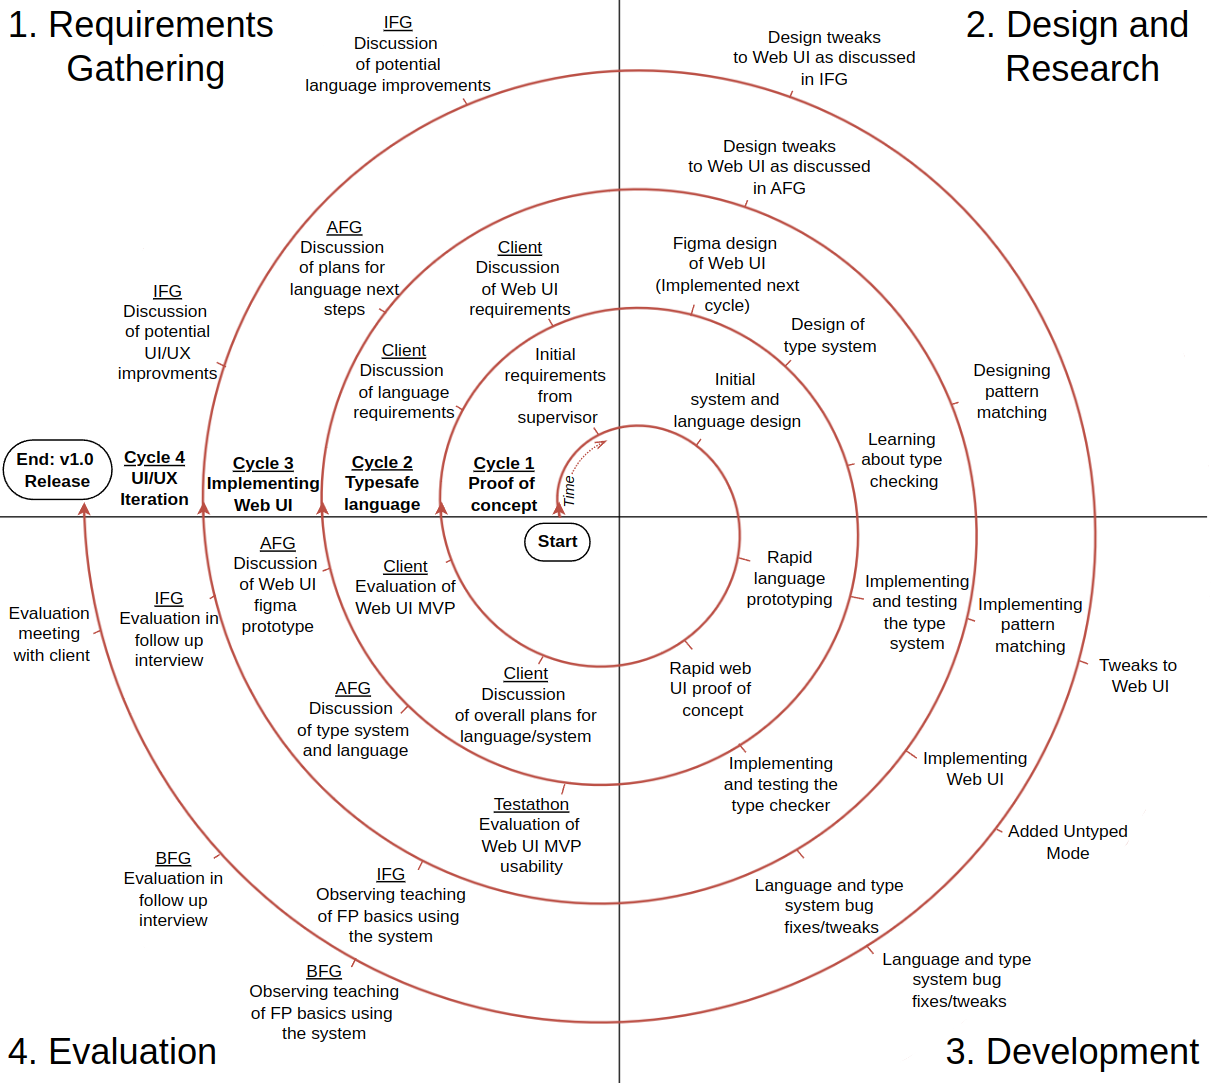
\includegraphics[width=0.98\linewidth]{images/spiral1.drawio.png}}
    \caption{A spiral representation of the project lifecycle, showing the 4 iterations, and the work done in each part of each phase. }\label{fig:spiral}
\end{figure}

This iterative methodology helped manage complexity and uncertainty. Getting frequent feedback from focus groups 